% --------------------------------------------------------------
% This is all preamble stuff that you don't have to worry about.
% Head down to where it says "Start here"
% --------------------------------------------------------------
 
\documentclass[12pt]{article}
 
\usepackage[margin=1in]{geometry} 
\usepackage{amsmath,amsthm,amssymb,algpseudocode,listings}
\usepackage{color}
\usepackage{DejaVuSansMono} 
\usepackage{setspace}
\usepackage{parskip}
\usepackage{graphicx}


\definecolor{Code}{rgb}{0,0,0}
\definecolor{Decorators}{rgb}{0.5,0.5,0.5}
\definecolor{Numbers}{rgb}{0.5,0,0}
\definecolor{MatchingBrackets}{rgb}{0.25,0.5,0.5}
\definecolor{Keywords}{rgb}{0,0,1}
\definecolor{self}{rgb}{0,0,0}
\definecolor{Strings}{rgb}{0,0.63,0}
\definecolor{Comments}{rgb}{0,0.63,1}
\definecolor{Backquotes}{rgb}{0,0,0}
\definecolor{Classname}{rgb}{0,0,0}
\definecolor{FunctionName}{rgb}{0,0,0}
\definecolor{Operators}{rgb}{0,0,0}
\definecolor{Background}{rgb}{0.98,0.98,0.98}

\lstnewenvironment{python}[1][]{
\lstset{
numbers=left,
numberstyle=\ttfamily,
numbersep=1em,
xleftmargin=1em,
framextopmargin=2em,
framexbottommargin=2em,
showspaces=false,
showtabs=false,
showstringspaces=false,
frame=l,
tabsize=4,
% Basic
basicstyle=\ttfamily\small\setstretch{1},
backgroundcolor=\color{Background},
language=Python,
% Comments
commentstyle=\color{Comments}\slshape,
% Strings
stringstyle=\color{Strings},
morecomment=[s][\color{Strings}]{"""}{"""},
morecomment=[s][\color{Strings}]{'''}{'''},
% keywords
morekeywords={import,from,class,def,for,while,if,is,in,elif,else,not,and,or,print,break,continue,return,True,False,None,access,as,,del,except,exec,finally,global,import,lambda,pass,print,raise,try,assert},
keywordstyle={\color{Keywords}\bfseries},
% additional keywords
morekeywords={[2]@invariant},
keywordstyle={[2]\color{Decorators}\slshape},
emph={self},
emphstyle={\color{self}\slshape},
%
}}{}

\newcommand{\N}{\mathbb{N}}
\newcommand{\Z}{\mathbb{Z}}
 
\newenvironment{theorem}[2][Theorem]{\begin{trivlist}
\item[\hskip \labelsep {\bfseries #1}\hskip \labelsep {\bfseries #2.}]}{\end{trivlist}}
\newenvironment{lemma}[2][Lemma]{\begin{trivlist}
\item[\hskip \labelsep {\bfseries #1}\hskip \labelsep {\bfseries #2.}]}{\end{trivlist}}
\newenvironment{exercise}[2][Exercise]{\begin{trivlist}
\item[\hskip \labelsep {\bfseries #1}\hskip \labelsep {\bfseries #2.}]}{\end{trivlist}}
\newenvironment{problem}[2][Problem]{\begin{trivlist}
\item[\hskip \labelsep {\bfseries #1}\hskip \labelsep {\bfseries #2.}]}{\end{trivlist}}
\newenvironment{question}[2][Question]{\begin{trivlist}
\item[\hskip \labelsep {\bfseries #1}\hskip \labelsep {\bfseries #2.}]}{\end{trivlist}}
\newenvironment{corollary}[2][Corollary]{\begin{trivlist}
\item[\hskip \labelsep {\bfseries #1}\hskip \labelsep {\bfseries #2.}]}{\end{trivlist}}


\lstset{basicstyle=\footnotesize\ttfamily,breaklines=true}
\lstset{framextopmargin=50pt,frame=bottomline}

\begin{document}
 
% --------------------------------------------------------------
%                         Start here
% --------------------------------------------------------------
 
\title{Homework 6}%replace X with the appropriate number
\author{Jeremy Wright\\ %replace with your name
CSE598 - Analysis of Algorithms} %if necessary, replace with your course title
 
\maketitle
\begin{problem}{8.1a}
    Yes, there might be a reduction from interval scheduling to vertex cover,
    however, this reduction is useless. Interval scheduling has a known
    polynomial time algorithm, thus, if we ``reduce''an easy problem to a hard
    problem we have only created more work for ourselves.
\end{problem}

\begin{problem}{8.1b}
    Independent set reduces to Interval scheduling? Unknown since that would
    answer P vs. NP.  Independent Set is NP hard. Interval scheduling has
    a polynomial time algorithm so if there was a reduction then P= NP.
\end{problem}

\begin{problem}{8.3}
    Vertex cover reduces to Efficient Recruiting. At each ode is a counselor. The
    edge from the node is the sport the counselor can over. For sports handled
    by a single counselor, draw an edge back to the same counselor.
    
    We can enumerate the
    edges and vertexes in polynomial ($O(n)$) time. So solving the Vertex cover
    will result in a solution to the efficient recruiting problem.

    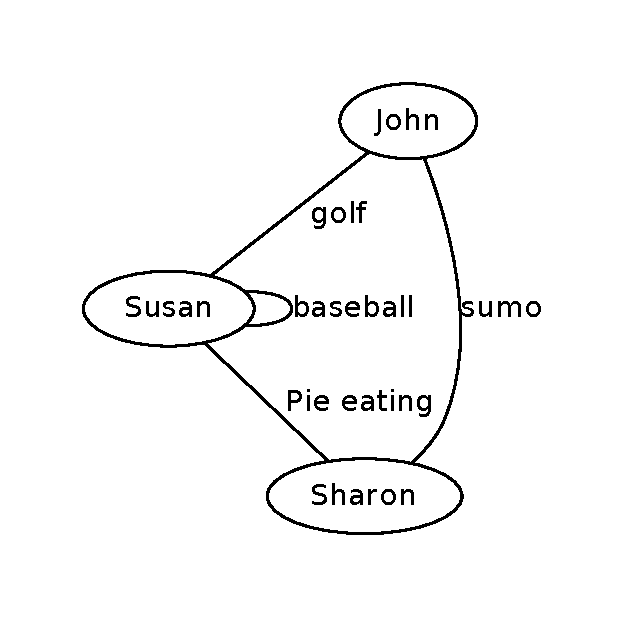
\includegraphics[width=0.8\textwidth]{recuruiter.pdf}

    Notice in this example, that Susan is the only counselor that can teach
    baseball. Thus the resulting graph \emph{must} include Susan's node,
    similarity, Susan must be hired by the camp, if they wish to teach baseball.
    Our reduction seems robust.
\end{problem}

\begin{problem}{8.5}

    $A = \{a_1, a_2, \dots , a_n \}$

    $B = \{B_1, B_2, B_3\dots \}$

    Hamiltonian Circuit reduces to Hitting Set Problem.

    Hamiltonian Circuit requires a path runs through all nodes of the graph once. 

    Each node in the hamiltonian graph replaces an object A, i.e. $a_1,
    a_2, \dots$.  Each subset B contains the edges to connect nodes. If
    a hamiltonian path exists, then there is a subset B, that hits all edges in
    A. Also, it is trivial to see that this translation takes polynomial time.
    Therefore, hitting path is NP complete.
\end{problem}

\begin{problem}{8.20}
    Reduce the graph coloring problem, to low diameter.

    Graph coloring can be reduces in polynomial tie to the low diameter
    clustering problem. Vertices represent the set of points $p_1, p_2,
    p_3\dots$.  and the edges represent the sets $\{p_i, p_j\}$ color the nodes
    with k colors. Each color represents a partition set. Since the colors
    repeat as soon as possible, without being adjacent, the partition set will
    be as small a diameter as possible, and overall a minimum.

    Translating the sets to nodes, and edges takes liner time, and thus is
    polynomial.
\end{problem}

\begin{problem}{Set Partitioning}
    $\text{subset sum} \le_p \text{Set Partition}$
We can see that Set partition has a non-deterministic solution by: Guess the
partition of integers. Sum the integers and verify the sum is equal. Summing the
integers is polynomial in time, and non-deterministically we can guess the
correct partition.


\end{problem}

\begin{problem}{0-1 integer programming}
$\text{3 SAT} \le_p \text{0-1 integer programming}$
Let integers be a set $\{i_1, i_2, i_n\}$.

Boolean values correspond to integer values of 0 or 1.

Let all correspond to  $(x_1, x_2, x_n <=> i_1, i_2, i_3)$

For each truth clause we setup a corresponding inequality. For example, the
truth clause $x_1 + \bar{x_2} + x_3$ we translate to $i_1 + (1 - i_2) + i_3 \ge
1$.
For each not we subtract the factor from 1. In this way we can represent all
boolean clauses as integer inequalities. This translation is linear in the
number of boolean terms, thus we do not perform an exponential amount of work
in our reduction. 

\end{problem}

\end{document}
